\label{chap_kmc400}

The Kangaroo foundation has contributed significantly to the development of this project. The experts that work with the foundation have provided us information on their research methodologies. They also provided us two very interesting data-sets and were willing to test all our prototypes. In return we helped them analyze and make sense of these complex data-sets. This collaboration enriched the project and allowed the experts in the foundation to extract information from the data efficiently. This chapter will illustrate the benefits of this collaboration and show how the Braviz platform can provide value in a real study. Notice that the full methodology and results from this study can be found elsewhere \autocite{KMC400}; in this chapter only some aspects are illustrated in order to provide the context in which the tools were used.

Charpak N., Ruiz JG., Tessier R., Hernandez JT., Uriza LF., Teillaud S. Final Report of the Project : Randomized open controlled trial on Kangaroo Mother Care Vs Traditional Care for Low Weight Birth infants. Patients-centered outcomes at the age of 18 years. 2015

\section{Background}


- What is KMC

%- The first randomized trial
Between 1993 and 1996 a randomized controlled trial comparing short and middle term outcomes of KMC in comparison to traditional treatment. The sample consisted of 746 infants born with low weight (less than 2000g.) at \emph{Clinica San Pedro Claver} in Bogotá \autocite{charpak_current_1996,charpak_kangaroo_1997,charpak_randomized_2001,charpak_kangaroo_2005}. Elligible infants were randomly assigned to the KMC or traditional intervention. KMC group was on kangaroo position 24 hours a day and fed by breast feeding with an optional supplement (preterm infant formula) derived by spoon or dropper in order to guarantee a weight gain of 15 grams per kilogram per day until the reach of term. Children in the traditional group were kept in an incubator until they were able to control their temperature and are gaining weight at an acceptable rate. Infants were discharged according to standard hospital practice. Both groups were followed until one year of corrected age. 

%-- What were the main findings

During this year there were fewer deaths in the KMC group as well as fewer visits to the hospital caused by infections. In addition mothers from the KMC group felt more competent. Griffiths and INFANIB tests showed higher development in the KMC group. The effect was more prominent on those born before 32 weeks of gestational age and those who went trough ICU. There was also a high impact of KMC on the development of personal relations and on planning functions related to brain development \autocite{tessier_kangaroo_2003}.

%\autocite{charpak_kangaroo_1997}
%\autocite{charpak_kangaroo_2005}
%\autocite{charpak_randomized_2001}
%\autocite{charpak_current_1996}

%(preguntar a Rejean y Nathalie)
-- Findings from other studies
-- KMC in the world

\section{Pilot Study}

In 2009, thirty-nine children who were part of the original study were relocated. The sample was composed of children born at or before 33 weeks of gestational age, 21 belonged to the KMC group and 18 from the traditional group. In addition, 9 kids born at term at the same hospital were recruited. These kids went trough

What tests



The pilot study
 - Data
 - TMS findings
 - IMAGINE


\section{Saving Brains Project}

%Teams : images, psycho, economists, medical, eyes, social workers, 


%The saving brains project

Between 2013 and 2014, with financing from Canada Grand Challenges, a sample of X subjects from the original study was retrieved. By this time the participants were between 18 and 20 years old. The study aimed at identifying if the KMC intervention had a long term effect protecting the brain against cognitive, social, and academic difficulties. Specifically, by analyzing data about  brain maturation and structure, mental functions and behavioral patterns exhibited in family, school and work. The data collected in this project is 

AGREGAR REFERENCIAS

\begin{itemize}
	\item Cognitive
	\begin{itemize}
		\item WASI II: Abbreviated intelligence test
		\item TAP: Attention test
		\item CVLT: Verbal learning test
	\end{itemize}
	\item Life Quality
	\begin{itemize}
		\item Kidscreen: Health related quality of life questionnaire.
		\item Life habits questionaire: ???????
		\item Pediatric Quality of Life Inventory : ??????????
	\end{itemize}
	\item Mental Health
	\begin{itemize}
		\item CES-D: Depression self report
		\item Conners: ??????????????????????		
	\end{itemize}
	\item Behavior
	\begin{itemize}
		\item ABCL: Behavior checklist, completed by parents and best friend
		\item ASR: Acute stress response
		\item Rosemberg: Self-esteem questionnaire
		\item Apego ?????????????
	\end{itemize}
	\item Neurosensorial 
	\begin{itemize}
		\item Optometry: Full sight evaluation
		\item Audiometry: Full hearing evaluation
		\item Edimburg laterality inventory: Dominant hand for multiple tasks
		\item Nine Holes Peg Test: Manual dexterity
		\item Beery Visuo-Motor Integration: Assesses integration between visual and motor abilities by copying images from a booklet.
	\end{itemize}
	\item Environment
	\begin{itemize}
		\item ?????????????????
	\end{itemize}
	\item Academic Performance
	\begin{itemize}
		\item ICFES: Results from the state high-school evaluation
		\item School performance: Data of how the kids performed at school.
		\item Current activity: Are the kids working or studying? If they work, what kind of work? what is the wage?
	\end{itemize}
	\item TMS % ¿Se aplicó a todos?
	\begin{itemize}
		\item Rest motor threshold
		\item MEP (Motor Evoked Potential) Latency
		\item Intra-cortical inhibition
		\item Intra-cortical facilitation
		\item Inter-hemispheric inhibition
	\end{itemize}
\end{itemize}

% Hablar algo más de las variables psicológicas y clínicas como un todo


Additionally all variables captured during the first year follow up are available, this includes

\begin{itemize}
\item Social characteristics of parents
\item Pregnancy characteristics 
\item Type of birth
\item Weight, size and cranial perimeter at birth and during follow up
\item Hospitalization at birth and during follow up
\item Questionnaire of mother competence
\end{itemize}

Furthermore, kids who were born with high risk (less than 1700g.) went trough MRI scans. The protocols used were:

\begin{itemize}
	\item Clinical T1, T2, Flair
	\item MPRAGE
	\item DWI
	\item fMRI	
\end{itemize}

% - Data dimensions
% -- Clinical
% -- Psychology
% -- TMS
% -- MRI


EXPLAIN WHAT IS THE MAIN DATABASE (SPSS OR ACCESS)



 - Objectives
 - Data Collection
 -- Process
 --- how?
 --- when?
 -- Participants

 
 - Data Processing
 -- Pipeline
 -- Quality Control
 --- Early assessment
 --- Processing errors
 --- Pathologic Data
 -- Bundles Statistics
 -- Geometric descriptors

 - Exploratory Analysis
 -- Use cases with Nathalie
 -- Examples of obvious and non obvious findings

\subsection{TMS}
%TMS details
TMS examination was carried out using two Magstim 200 stimulators coordinated by the Magstim Bistim. Subjects were comfortably sited in a chair with the arm in a pillow. An electrode connected to a EMG was connected to the first dorsal interosseus muscle. The TMS coil was located on top of the motor area of the opposed hemisphere. Optimal location for the coil was determined by the operator by searching the location that would induce a higher response on the EMG. For this procedure the stimulator was configured at 80\% of maximum output, if the hotspot could not be found at this level output power would be raised. The next step was estimating the motor threshold, this is, the minimum output power required in order to induce a response in the muscle on half the attempts. A test was next performed at 120\% of the threshold, this output would be used as baseline for the next steps.

Intracortical inhibition was tested by applying two pulses, the first one at 80\% of the threshold and the second one at 120\% of the threshold, both pulses would be separated by 3ms. For testing intracortical facilitation two pulses, at 80\% and 120\%, were used, but in this case separated by 15ms. These tests were repeated 10 times each, and performed on both hemispheres.

For testing interhemispheric inhibition the subject was asked to apply pressure with the thumb, first at maximum strength, and then maintaining it at 50\% of the maximum level. Afterwards a single, at 200\% of the motor threshold ,pulse would be applied on the same side as the target muscle, this pulse would generate a responde on the opposite side but also would cause an inhibition in the active muscle. 

%TMS processing


\subsection{MRI Imaging}

%Autocite reporte interno Pablo y Felipe

MRI image acquisition was done at the San Ignacio University Hospital using a Phillips Achieva tree Tesla scanner with a eight channels head  antenna. A sequence resembling MPRAGE was captured in order to provide freesurfer the best images it can handle. Additionally a volumetric T1 image and a Flair sequence were captured to provide additional anatomical context. In addition a high quality diffusion weighted sequence was captured as one of the main goals of the study was analyzing white matter. Tables \ref{tab_mri_params} and \ref{tab_fmri_params} show the acquisition parameters used for each sequence. 
\begin{table}
	\centering
	\footnotesize
		\begin{tabular}{l|rrrrr}
				Sequence&MPRAGE	&Flair	&T1 3D &DWI\\ \hline				
				Sequence Type	&GR	&IR	&GR &SE\\ 
				Dimensions	&3	&2	&3 &2\\
				Slice width	&1	&5.5	&1 &2\\
				Repetition time	&8.52	&11000	&7.76 &8610\\
				Eco time	&4.13	&125	&3.724 &83.41\\
				Slice spacing	&1	&6.5	&0.5 &2\\
				Phase Encoding Steps	&251	&243	&220 &112\\
				Echo train length	&187	&31	&220 &59\\
				Filed of view	&74	&100	&100 &100\\
				Reconstruction	Diameter&250	&220	&220 &224\\\hline
				Dimension x &250	&1024 &448  &128 \\
				Dimension y &256	&1024 &448 &128 \\
				Dimension z &160	&23 &310 &70 \\ \hline
				Voxel Size x	&0.97 &0.49 &0.21  &1.75 \\
				Voxel Size y	&0.97 &0.49 &0.21 &1.75 \\
				Voxel Size z	&1  &0.5 &6.5 &2 \\ \hline
				Gradients   &    &    &    &    32 \\
		\end{tabular}
	\caption{MRI sequences acquisition parameters}
	\label{tab_mri_params}
\end{table}


\begin{table}
	\centering
	\footnotesize
		\begin{tabular}{l|rrrrr}

	Paradigm &Attention	&Coordination	&Memory	&Grip &Fear\\ \hline
	Sequence Type	&GR	&GR	&GR	&GR &GR\\
	Volumes	&90	&90	&128	&125 &495\\
	Dimensions	&2	&2	&2	&2 &2\\
	Slice width	&3	&3	&3	&3 &3\\ \hline
	Repetition time	&2000	&2000	&4000	&2000 &2300\\
	Eco time	&28	&28	&28	&28 &30\\
	Slice spacing	&3	&3	&3	&3 &3\\
	Phase Encoding Steps	&80	&80	&80	&80 &80\\
	Echo train length	&43	&43	&43	&43 &43\\
	Filed of view	&100	&100	&100	&100 &100\\
	Reconstruction	Diameter&240	&240	&240	&240 &240\\ \hline
	Dimension x &80	&80 &80 &80 &64 \\
	Dimension y &80	&80 &80 &80 &64 \\
	Dimension z &40	&40 &40 &40 &32 \\ \hline
	Voxel Size x	&3 &3 &3 &3 &3.8 \\
	Voxel Size y	&3 &3 &3 &3 &3.8 \\
	Voxel Size z	&3 &3 &3 &3 &3 \\
		\end{tabular}
	\caption{Functional MRI sequences acquisition parameters}
	\label{tab_fmri_params}
\end{table}

Five f-MRI paradigms were used in this study: Attention, coordination, memory, grip and fear. Because each participant could only remain inside the scanner for a limited time, not all paradigms could be applied to all subjects. Two groups were created, the first one went trough grip, coordination, attention and memory; while the second one trough grip, coordination and fear. 

The grip paradigm had a block design where subjects were asked to apply pressure with thumb on the side of the index finger, and in this way activating the first dorsal interosseus muscle, the muscle targeted in the TMS test. The coordination paradigm also had a block design but this time the task was opening and closing one or both hands following the pictures presented in the screen. The attention used a block design as well, in this case the subject would be presented with seven points on the screen, and they were instructed to follow the tree red points that blink. Afterwards all points would become black and start moving around the screen. At the end the initial points would become red again and the participant would be asked if they arrived to the same final position. 
The memory paradigm was composed of two stages, both in block designs. During the first stage participants were shown couples of words and asked to memorize them. During the second stage participants were presented with a word they have seen before, and two other words. They were asked to identify from the two options, which word was seen before with together with the first word.

¿POR QUE SE HICIERON ESTOS PARADIGMAS?

The fear conditioning paradigm \autocite{FRANCOISES} was event related and divided in two stages. In the first stage participants were randomly presented with two woman faces. Additionally half of the time one of the faces was shown, it was accompanied by a loud scream.  During the second stage  both faces were shown again randomly, but this time there would not be any scream. After the presentation of each face at both stages participants would have to respond using a qualitative scale how anxious they were feeling.
\smallskip

% Data analysis
Image data was pre-processed as described in section \ref{sec_preproc}. Anatomical images went trough a VBM analysis using SPM comparing the two groups from the randomized study, using age and gender as control variables. Additionally \emph{Eigenvariants} for each subject in each region of interest were extracted and added to the database of variables. MPRAGE images went trough the FreeSurfer recon-all pipeline and all output statistics (volumes, cortical thickness, surface areas, and cortex curvature) were added to the database. 

At this points all of the spatial artifacts generated by freesurfer were also available in Braviz, and therefore it was easy to use python scientific libraries to perform additional analyzes. We created a script that went trough all segmented structures, and for each one calculated the main, second and third axes, as shown in figure \ref{fig_jth_descs}. The lengths of these axes were added to the database as new variables.

% JTHP descriptors
\begin{figure}
	\centering
		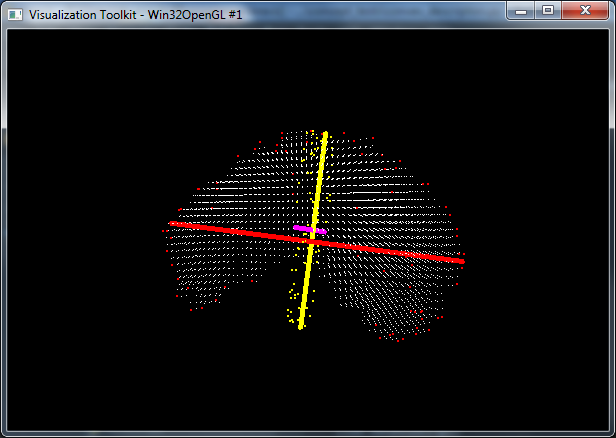
\includegraphics[width=\textwidth]{figures/kmc400/desc_4}
	\caption{Illustration of the geometric descriptors calculated in python, white dots are the center of voxels that belong to a given structure, red points are those in the convex hull, the red line is the mayor axis of the structure, yellow points are the points in the structure projected to a plane perpendicular to the main axis, the yellow line is the mayor axis of this plane, finally the purple line is the axis perpendicular to the red and yellow axes.}
	\label{fig_jth_descs}
\end{figure}

DWI data was processed using Camino and the Free Surfer brain masks as references. Transformations between diffusion space and structural MRI space were calculated using \emph{FSL FLIRT}. From Camino we obtained FA, MD and color DTI maps, as well as full brain tractography. All of these were integrated into Braviz and made available for the experts. Additionally by using python scientific libraries and vtk we were able to combine Free Surfer data with tractography in order to isolate bundles going trough particular structures. Mean FA, mean MD, mean length and number of tracks in the bundle were extracted for each bundle of interest.  While this could be achieved without Braviz, it was certainly easier using the infrastructure provided by the software. Additionally Braviz was used to let experts define spherical regions of interests and, based no them, define additional bundles of interest. The same scalar metrics mentioned before were extracted for these bundles. 

Additionally DWI data was processed using Free Surfer's Tracula. Output statistics were exported into the database and the probability maps of the bundles were integrated into Braviz for visualization. 

Functional MRI data was pre-processed in SPM.  After that a first level analysis was performed using specific contrasts for each paradigm, followed by a second level analysis using the main groups as regressor. The results from this analysis can be seen in \autocite{PABLO_FELIPE}. The Braviz \emph{fMRI Explore} tool was particularly useful in the first level stage as it displayed contrasts in a direct and clear way. Figure \ref{fig_spm_contrast_error} shows a problem with a contrast, because the left and right conditions are not of the same length. This problem was quickly identified and corrected.

\begin{figure}
	\centering
		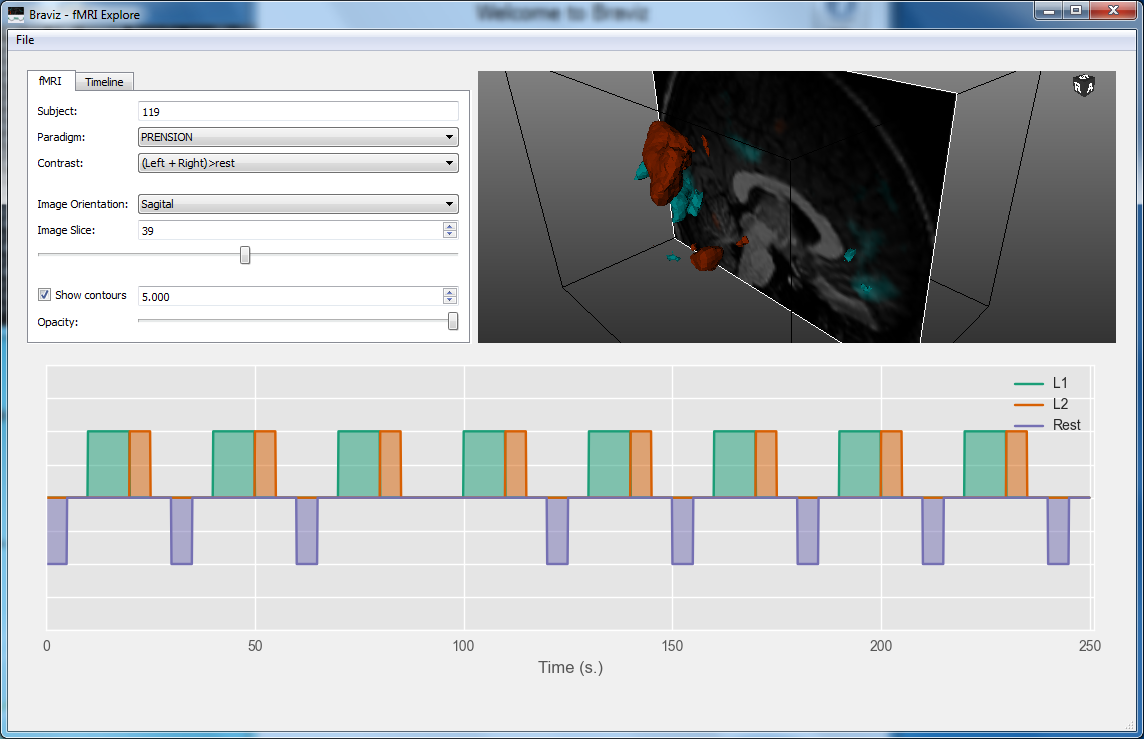
\includegraphics{figures/kmc400/erroro_fmri2}
	\caption{A problematic f-MRI contrast, L1 and L2 should have the same length.}
	\label{fig_spm_contrast_error}
\end{figure}
 

\subsection{Economics}

The Research Group in Economics from Universidad del Rosario got involved in the project in order to analyze the education and work history of the cohort. The main question for the group was finding if the kmc intervention had effects on educational and work outcomes.  For this purpose they created a questionnaire, based on validated questions from previous studies and the National Department of Statistics (DANE). This questionnaire was applied to each participant at the end of the domiciliary visit. This instrument inquired about the schools to which the participant attended, the performance in those schools, if currently the participant was studying or working, what kind of studies were they pursuing and what kind of work were they performing. Participants were reminded that the information collected was only for research purposes and that data that could identify them would never be published. The questionnaires were tabulated by a professional at the foundation and verified by the Economics group. Finally the results were merged with the other variables of the study.

Additionally participants gave their authorization to fetch the results of the last state high-school test (Saber-11) they completed. This test is applied to all students of the country when they are about to finish high-school, and it comprises sections on mathematics, language, social studies, natural sciences and English.

Analysis began by taking a broad look of the effect of the intervention on key variables, as the current age and performance in Saber-11. This was done using linear regression in the Stata software. At the next stage the analysis was performed using additional variables as controls. These variables were chosen based on economics theory and previous experience of main researchers. This stage showed some apparent contradictions in the results, which were discussed with the rest of the Kangaroo team. From this discussions ideas of possible explanations and additional variables that should be taken into effect emerged. This ideas were tested against the data with positive results. 

It must be noticed that the analysis was carried out mainly trough tables generated by Stata. Generating graphics in this software required additional steps, and therefore was done only to create the results.

¿HUBIERA AYUDADO TENER ACCESO A BRAVIZ DESDE EL COMIENZO?


The complete discussion of the methodology and results from the Economics team can be found in \autocite{?}



\subsection{Specific Braviz contributions}

quality control
fibers analysis
sharing, presentations

